\chapter{CƠ SỞ LÝ THUYẾT}
\label{chapter:co_so_ly_thuyet}

Chương này hệ thống hóa các cơ sở lý thuyết và nguyên lý khoa học nền tảng làm tiền đề cho việc thiết kế, xây dựng và đánh giá hệ thống trợ lý học tập thông minh. Nội dung trọng tâm bao gồm: tổng quan về xử lý ngôn ngữ tự nhiên và trí tuệ nhân tạo tạo sinh, kiến trúc và cơ chế hoạt động của các mô hình ngôn ngữ lớn, phương pháp sinh tăng cường truy xuất RAG, hệ quản trị cơ sở dữ liệu vector, các kỹ thuật biểu diễn đa phương thức, cùng các giải pháp truy xuất lai và kỹ thuật tái xếp hạng tương tác chéo.

\section{Tổng quan về Xử lý ngôn ngữ tự nhiên và Trí tuệ nhân tạo tạo sinh}
Xử lý ngôn ngữ tự nhiên là một phân ngành nền tảng của trí tuệ nhân tạo, hướng tới mục tiêu phát triển các phương pháp và mô hình tính toán cho phép máy tính có khả năng tiếp nhận, giải mã cú pháp, thấu hiểu ngữ nghĩa và tạo lập ngôn ngữ con người một cách tự nhiên. Lịch sử phát triển của lĩnh vực này ghi nhận sự dịch chuyển mang tính bước ngoặt: từ các hệ thống dựa trên tập luật hình thức thủ công và các mô hình thống kê tần suất sang các kiến trúc học sâu hiện đại~\cite{bengio2003neural, lecun2015deeplearning}. Bước đột phá khởi đầu cho giai đoạn này là sự xuất hiện của các phương pháp biểu diễn ngữ nghĩa phân tán trong không gian vector liên tục, tiêu biểu như mô hình word2vec~\cite{mikolov2013word2vec}, từ đó mở đường cho các kiến trúc mạng nơ-ron hồi quy và mô hình biến đổi chuỗi sang chuỗi tích hợp cơ chế chú ý phục vụ dịch máy tự động~\cite{sutskever2014seq2seq, bahdanau2015attention}.

Trên cơ sở đó, sự bùng nổ của trí tuệ nhân tạo tạo sinh đã thiết lập một bước chuyển biến sâu sắc về năng lực ứng dụng thực tiễn. Khác với các mô hình phân biệt truyền thống vốn chỉ tập trung ước lượng xác suất có điều kiện nhằm phân loại hoặc nhận dạng các mẫu dữ liệu có sẵn, các mô hình tạo sinh học phân phối xác suất đồng thời trên tập dữ liệu huấn luyện, cho phép tổng hợp và khởi tạo những đối tượng dữ liệu hoàn toàn mới mang tính nhất quán cao về mặt ngữ nghĩa, bao gồm văn bản, hình ảnh, âm thanh và mã nguồn phần mềm~\cite{bommasani2021foundation}. Trong không gian dữ liệu văn bản, nhân tố đóng vai trò hạt nhân thúc đẩy cuộc cách mạng này chính là các mô hình ngôn ngữ lớn~\cite{zhao2023llmsurvey}.

\section{Mô hình ngôn ngữ lớn}
\subsection{Kiến trúc Transformer và cơ chế tự chú ý}
Được công bố bởi Vaswani và các cộng sự vào năm 2017~\cite{vaswani2017attention}, kiến trúc Transformer đã nhanh chóng thay thế các mô hình tuần tự truyền thống để trở thành cấu trúc nền tảng cho hầu hết các mô hình ngôn ngữ lớn hiện đại. Trọng tâm của Transformer là cơ chế tự chú ý đa điểm, cho phép mô hình tính toán đồng thời trọng số tương tác giữa từng từ tố với toàn bộ các từ tố còn lại trong ngữ cảnh, hoàn toàn không bị giới hạn bởi khoảng cách vị trí giữa chúng.

Cơ chế này khắc phục triệt để hiện tượng suy giảm gradient và hạn chế mất mát thông tin ngữ cảnh xa vốn xuất hiện phổ biến ở các mạng hồi quy như RNN hay LSTM. Đồng thời, kiến trúc Transformer giải phóng năng lực tính toán song song quy mô lớn trên các bộ xử lý đồ họa, tạo điều kiện tiên quyết cho việc mở rộng quy mô dữ liệu và tham số huấn luyện lên tới hàng trăm tỷ trọng số. Từ cấu trúc Transformer, hai nhánh mô hình tiền huấn luyện chủ đạo đã phát triển mạnh mẽ: nhánh bộ mã hóa hai chiều tiêu biểu như BERT~\cite{devlin2019bert} tối ưu cho các bài toán phân loại và thấu hiểu ngữ nghĩa; và nhánh bộ giải mã tự hồi quy như dòng GPT~\cite{brown2020gpt3} chuyên biệt cho tác vụ tạo lập văn bản nối tiếp. Các nghiên cứu định lượng đã khẳng định rằng khi mở rộng quy mô tham số, thể tích dữ liệu và năng lực tính toán, chất lượng mô hình tuân theo các quy luật tỷ lệ chặt chẽ~\cite{kaplan2020scaling}, làm bộc lộ những năng lực suy luận phức tạp mà các mô hình quy mô nhỏ không thể đạt được~\cite{wei2022emergent}.

\subsection{Họ mô hình ngôn ngữ lớn Qwen}
Trong số các dòng mô hình ngôn ngữ lớn mã nguồn mở hiện nay, họ mô hình Qwen, tiêu biểu là thế hệ Qwen2.5 do Alibaba Cloud phát triển~\cite{qwen25_2024}, được đánh giá là một trong những giải pháp dẫn đầu về hiệu năng tổng thể. Sự phát triển mạnh mẽ của các dòng mô hình mã nguồn mở như LLaMA~\cite{touvron2023llama} hay Qwen mang lại cho cộng đồng nghiên cứu khả năng tự chủ công nghệ cao, cho phép triển khai hoàn toàn cục bộ, bảo mật dữ liệu và tùy biến chuyên sâu mà không bị lệ thuộc vào các giao diện lập trình thương mại đóng kín.

Trong khuôn khổ đồ án, phiên bản \textbf{Qwen2.5-3B-Instruct} được lựa chọn làm mô hình sinh ngôn ngữ nòng cốt. Mô hình được tinh chỉnh chuyên sâu theo chỉ thị kết hợp phương pháp học tăng cường từ phản hồi của con người~\cite{ouyang2022instructgpt}, đem lại năng lực tuân thủ chỉ thị và lập luận vượt trội trong phân khúc mô hình nhỏ gọn với quy mô khoảng 3 tỷ tham số. Kích thước tối ưu này cho phép hệ thống đáp ứng tốt các bài toán thực tế trên cơ sở hạ tầng có tài nguyên tính toán giới hạn mà vẫn bảo đảm tốc độ suy luận nhanh và chất lượng văn bản sinh ra mạch lạc. Toàn bộ quy trình thực nghiệm và kiểm thử của đồ án được triển khai thống nhất trên máy trạm chỉ sử dụng \textbf{CPU} (chi tiết tại Bảng~\ref{tab:env}). Đặc biệt, mô hình Qwen2.5 thể hiện năng lực đa ngữ xuất sắc, thấu hiểu và diễn đạt tiếng Việt trôi chảy, chuẩn xác, đáp ứng tốt yêu cầu giải thích kiến thức khoa học mang tính sư phạm trong môi trường giáo dục Việt Nam~\cite{nguyen2020phobert}.

\section{Sinh tăng cường truy xuất RAG}
\subsection{Những hạn chế cố hữu của mô hình ngôn ngữ lớn độc lập}
Mặc dù thể hiện khả năng biểu đạt ngôn ngữ rất tự nhiên, các mô hình ngôn ngữ lớn khi triển khai độc lập đều bộc lộ ba điểm nghẽn kỹ thuật căn bản~\cite{gao2023ragsurvey}:
\begin{enumerate}
    \item \textbf{Ảo giác tri thức:} Mô hình có thể tạo lập các khẳng định sai lệch hoặc suy đoán thiếu cơ sở thực tế với văn phong hết sức tự tin, thiếu sự đối sánh với dữ liệu xác thực~\cite{ji2023hallucination, huang2023hallucination}.
    \item \textbf{Tính chất tri thức tĩnh:} Toàn bộ tri thức của mô hình bị đóng băng tại thời điểm hoàn tất tập dữ liệu huấn luyện, không thể tự cập nhật thông tin mới trừ khi phải trải qua quá trình tái huấn luyện đòi hỏi chi phí tính toán vô cùng đắt đỏ~\cite{lewis2020retrieval}.
    \item \textbf{Sự thiếu hụt tri thức chuyên biệt:} Mô hình không có sẵn quyền truy cập vào các kho học liệu nội bộ, tài liệu đặc thù của tổ chức hay nội dung chi tiết của các bộ sách giáo khoa chuẩn mực quốc gia~\cite{guu2020realm}.
\end{enumerate}

\subsection{Nguyên lý hoạt động của kiến trúc RAG}
\label{sec:rag_nguyenly}
Kiến trúc sinh tăng cường truy xuất RAG~\cite{lewis2020retrieval} ra đời nhằm giải quyết triệt để các hạn chế trên thông qua sự kết hợp cộng sinh giữa hai thành phần: hệ thống truy xuất thông tin và mô hình tạo sinh ngôn ngữ. Thay vì xem mô hình ngôn ngữ như một kho lưu trữ tri thức tham số khép kín, mô hình RAG tách biệt thành phần ghi nhớ tri thức sang một cơ sở dữ liệu bên ngoài, xem mô hình ngôn ngữ lớn như một bộ xử lý suy luận hoạt động trên ngữ cảnh được cung cấp tức thời~\cite{guu2020realm, izacard2021fid, gao2023ragsurvey, asai2023selfrag, yan2024crag}.

\begin{figure}[H]
    \centering
    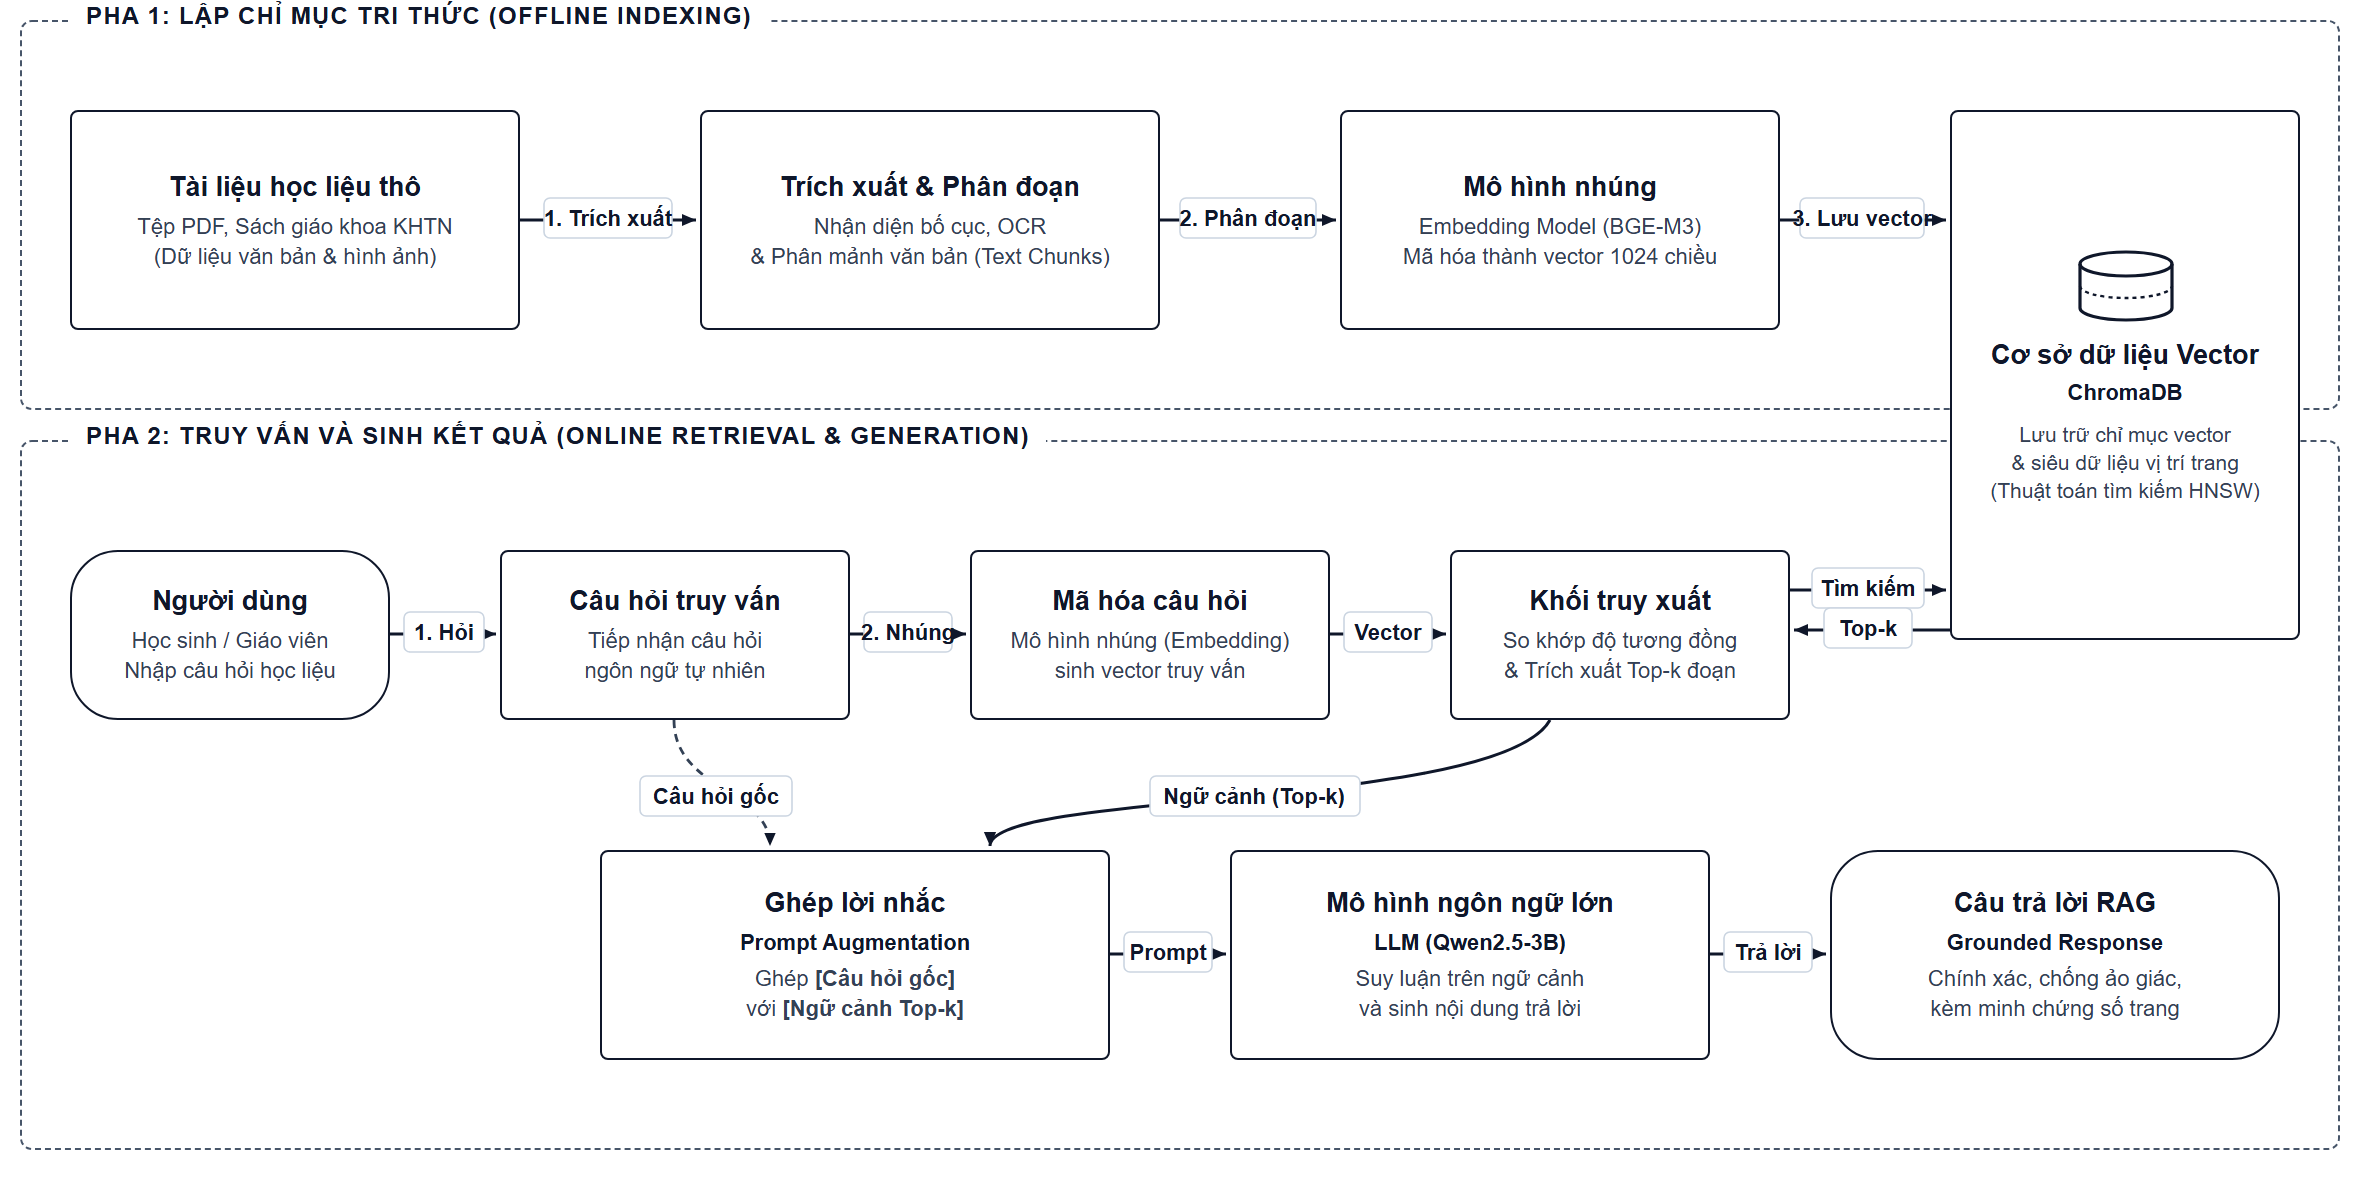
\includegraphics[width=\textwidth]{src/images/chapter2/rag_concept.png}
    \caption{Sơ đồ nguyên lý hoạt động cơ bản của hệ thống RAG (Nguồn: Tổng hợp từ~\cite{lewis2020retrieval, gao2023ragsurvey})}
    \label{fig:rag_concept}
\end{figure}

Quy trình vận hành chuẩn của một hệ thống RAG bao gồm hai pha chính (Hình~\ref{fig:rag_concept}):
\begin{itemize}
    \item \textbf{Pha Lập chỉ mục:} Dữ liệu tài liệu thô từ các tệp PDF và ảnh chụp trang sách được trích xuất và phân chia thành các đoạn văn bản độc lập. Tiếp đó, mô hình nhúng chuyển đổi các đoạn này thành các vector số học đa chiều để lưu trữ và lập chỉ mục trong cơ sở dữ liệu vector.
    \item \textbf{Pha Truy vấn và Tạo sinh:} Khi người dùng gửi câu hỏi, hệ thống tiến hành nhúng câu hỏi thành vector truy vấn tương ứng. Cơ chế tìm kiếm độ tương đồng trong cơ sở dữ liệu vector sẽ xác định các đoạn văn bản có độ tương đồng ngữ nghĩa cao nhất để trích xuất thành tập ngữ cảnh liên quan. Phương pháp này, hay còn được gọi là truy xuất ngữ nghĩa theo vector đặc~\cite{karpukhin2020dpr}, cho phép tìm kiếm chính xác nội dung đồng nghĩa ngay cả khi không có sự trùng khớp hoàn toàn về mặt từ khóa, khắc phục nhược điểm của các thuật toán so khớp từ khóa thuần túy như BM25~\cite{robertson2009bm25}. Cuối cùng, lời nhắc có cấu trúc kết hợp giữa ngữ cảnh tài liệu và câu hỏi gốc sẽ được đưa vào mô hình ngôn ngữ để tạo lập câu trả lời hoàn chỉnh có căn cứ học liệu rõ ràng.
\end{itemize}

\section{Mô hình nhúng và Cơ sở dữ liệu Vector}
\subsection{Kỹ thuật biểu diễn nhúng ngữ nghĩa}
Kỹ thuật nhúng là quá trình ánh xạ các thực thể ngôn ngữ như từ, câu, đoạn văn bản hoặc phi ngôn ngữ như hình ảnh vào một không gian vector thực liên tục đa chiều $\mathbb{R}^d$~\cite{mikolov2013word2vec}. Đặc tính quan trọng nhất của không gian nhúng là bảo toàn quan hệ ngữ nghĩa: các thực thể có nội dung hoặc ý nghĩa tương đồng sẽ nằm gần nhau trong không gian vector đa chiều, được định lượng thông qua các phép đo như độ tương đồng cosine. Đối với cấp độ câu và đoạn văn bản, các kiến trúc dựa trên Sentence-BERT~\cite{reimers2019sbert} cho phép trích xuất các vector biểu diễn ngữ nghĩa cô đọng và có khả năng so khớp trực tiếp với hiệu quả tính toán vượt trội.

Trong hệ thống nghiên cứu, mô hình \texttt{BAAI/bge-m3}~\cite{chen2024bgem3} được sử dụng để sinh các vector biểu diễn ngữ nghĩa với kích thước $1024$ chiều. Đây là mô hình đa ngữ tiên tiến được thiết kế hỗ trợ đồng thời ba cơ chế biểu diễn gồm vector đặc, vector thưa và đa vector biểu diễn, đồng thời có khả năng tiếp nhận độ dài ngữ cảnh lớn lên tới $8192$ token, rất phù hợp với đặc thù của các đoạn văn bản sách giáo khoa thường đi kèm công thức, ký hiệu khoa học và thuật ngữ định nghĩa.

So với các kiến trúc nhúng nông quy mô $384$ chiều như \texttt{MiniLM}~\cite{wang2020minilm}, mô hình \texttt{BAAI/bge-m3} thể hiện năng lực biểu diễn ngữ nghĩa vượt trội trên các bảng xếp hạng chuẩn MTEB~\cite{muennighoff2022mteb} và BEIR~\cite{thakur2021beir}, đặc biệt đối với các tác vụ truy xuất học liệu đa ngữ phức tạp. Về mặt nguyên lý toán học của không gian vector, các mô hình nhúng có số chiều khác nhau sẽ định hình các không gian mêtric hoàn toàn tách biệt, không thể chiếu trực tiếp hay tính toán độ tương đồng qua lại. Do đó, việc thiết lập một không gian vector $1024$ chiều đồng nhất xuyên suốt toàn bộ kho dữ liệu là yêu cầu tiên quyết nhằm đảm bảo tính chuẩn xác cho các hàm khoảng cách hình học.

\subsection{Hệ quản trị cơ sở dữ liệu vector ChromaDB}
Cơ sở dữ liệu vector là hệ quản trị dữ liệu chuyên dụng được tối ưu hóa cho bài toán lưu trữ và tìm kiếm vector lân cận gần đúng trên quy mô dữ liệu lớn. Khác với các cơ sở dữ liệu quan hệ truyền thống chỉ hỗ trợ so khớp chính xác, cơ sở dữ liệu vector cho phép thực hiện truy vấn tương đồng tốc độ cao dựa trên các chỉ mục đồ thị lân cận phân tầng HNSW~\cite{malkov2018hnsw} hoặc các thư viện tính toán tối ưu như FAISS~\cite{johnson2019faiss}.

Trong đề tài này, ChromaDB~\cite{chromadb2023} được lựa chọn làm cơ sở dữ liệu vector trung tâm. ChromaDB là một giải pháp mã nguồn mở linh hoạt, hỗ trợ vận hành cục bộ ở chế độ nhúng với hiệu năng cao mà không yêu cầu thiết lập máy chủ dịch vụ phức tạp, đồng thời tích hợp liền mạch với hệ sinh thái LangChain~\cite{langchain2022}, tạo điều kiện thuận lợi cho việc tổ chức, cập nhật và truy xuất các phân mảnh tri thức từ sách giáo khoa.

\section{Kỹ thuật xử lý Đa phương thức trong kiến trúc RAG}
Nội dung sách giáo khoa môn Khoa học tự nhiên chứa mật độ cao các đối tượng trực quan: sơ đồ cấu tạo cơ quan sinh học, chu trình chuyển hóa, sơ đồ mạch điện, đồ thị dao động, thiết bị thí nghiệm... Một hệ thống RAG thuần văn bản sẽ bỏ lỡ hoàn toàn các tri thức trực quan này. Do đó, việc mở rộng sang kiến trúc đa phương thức là một đòi hỏi tất yếu, dựa trên nền tảng của các mô hình Vision Transformer~\cite{dosovitskiy2021vit} và các kiến trúc liên kết ngôn ngữ -- thị giác hiện đại~\cite{radford2021clip, li2022blip, liu2024llava, li2023blip2, alayrac2022flamingo}, kế thừa các thành tựu từ bài toán hỏi đáp trực quan trên hình ảnh~\cite{antol2015vqa} và xử lý tài liệu đa phương thức~\cite{cui2021documentai, huang2022layoutlmv3}.

\subsection{Các mô hình trích xuất và biểu diễn thị giác}
Hệ thống tích hợp có chọn lọc các mô hình thị giác máy tính chuyên dụng:
\begin{itemize}
    \item \textbf{Mô hình OwlViT}\footnote{\texttt{google/owlvit-base-patch32}}~\cite{minderer2022owlvit}: Mô hình phát hiện vật thể không cần huấn luyện trước dựa trên điều kiện văn bản, được ứng dụng nhằm hỗ trợ xác định toạ độ hộp bao của các biểu đồ và hình ảnh trên trang sách trong các trường hợp không có nhãn văn bản cố định.
    \item \textbf{Mô hình CLIP}\footnote{\texttt{openai/clip-vit-base-patch16}}~\cite{radford2021clip}: Mô hình liên kết ngôn ngữ -- thị giác được tiền huấn luyện trên hàng trăm triệu cặp ảnh--văn bản. CLIP mã hoá hình ảnh thành vector $512$ chiều chung một không gian biểu diễn với câu hỏi văn bản, cho phép thực hiện tìm kiếm chéo giữa các phương thức thông qua độ tương đồng cosine.
    \item \textbf{Mô hình Vintern-1B}\footnote{\texttt{5CD-AI/Vintern-1B-v2}}: Mô hình thị giác--ngôn ngữ hỗ trợ tiếng Việt có khả năng tự động tạo chuỗi miêu tả văn bản từ hình ảnh cắt ra. Trong đề tài, mô hình này đã được đưa vào thử nghiệm thực tế; tuy nhiên, do vấn đề phát sinh ảo giác và chi phí tính toán cao trên CPU, hệ thống đã lựa chọn giải pháp trích xuất siêu dữ liệu trực tiếp từ văn bản gốc thay vì dựa vào chú thích tự sinh (trình bày chi tiết tại Chương~\ref{chapter:phuong_phap_thuc_hien}).
\end{itemize}

Thông qua sự kết hợp của các công nghệ trên, kiến trúc RAG đa phương thức của hệ thống đảm bảo khả năng đồng bộ hóa luồng tri thức giữa văn bản lý thuyết và dữ liệu hình ảnh, tạo tiền đề cung cấp ngữ cảnh học liệu toàn diện nhất cho mô hình sinh câu trả lời.

\section{Truy xuất lai và Kỹ thuật tái xếp hạng}
\label{sec:cosolythuyet_hybrid}
Truy xuất ngữ nghĩa dựa trên vector đặc tuy có năng lực nắm bắt ngữ cảnh tốt nhưng không phải là phương pháp tối ưu tuyệt đối trong mọi tình huống, đặc biệt là khi phải xử lý các truy vấn chứa ký hiệu chuyên ngành hoặc thuật ngữ cụ thể. Nhằm đạt được hiệu năng truy xuất tối ưu, hệ thống kết hợp ba kỹ thuật nền tảng sau:

\subsection{Truy xuất từ khóa theo vector thưa: Thuật toán BM25}
Okapi BM25~\cite{robertson2009bm25} là thuật toán xếp hạng tài liệu dựa trên mô hình xác suất thống kê tần suất từ khóa, là chuẩn mực trong lĩnh vực truy xuất thông tin cổ điển. Với một câu truy vấn $Q$ bao gồm các từ tố $\{q_1, q_2, \dots, q_n\}$ và một tài liệu $D$, hàm điểm số BM25 được xác định theo công thức:
\begin{equation}
\mathrm{BM25}(D, Q) = \sum_{i=1}^{n} \mathrm{IDF}(q_i) \cdot
\frac{f(q_i, D)\,(k_1 + 1)}{f(q_i, D) + k_1\left(1 - b + b\,\dfrac{|D|}{\mathrm{avgdl}}\right)}
\end{equation}
trong đó $f(q_i, D)$ biểu thị tần suất xuất hiện của từ $q_i$ trong tài liệu $D$; $|D|$ là độ dài tài liệu; $\mathrm{avgdl}$ là độ dài trung bình của toàn bộ các tài liệu trong tập dữ liệu; $\mathrm{IDF}(q_i)$ là nghịch số tần suất tài liệu của từ $q_i$; $k_1$ và $b$ là hai siêu tham số thực nghiệm kiểm soát mức độ bão hòa tần suất và mức độ chuẩn hóa theo độ dài tài liệu.

Điểm mạnh cốt lõi của BM25 là khả năng so khớp chính xác từng ký tự. Đối với môn Khoa học tự nhiên vốn chứa mật độ cao các công thức hóa học như \ce{H2SO4} hay \ce{Fe2O3}, ký hiệu vật lí hoặc tên riêng của các định luật, đây là một lợi thế quyết định: câu hỏi của người học đòi hỏi tài liệu trích xuất phải chứa chính xác chuỗi ký hiệu đó mà không bị pha loãng bởi phép xấp xỉ ngữ nghĩa. Ngược lại, hạn chế của BM25 là không thể nhận diện được các từ đồng nghĩa hoặc các cách diễn đạt khác nhau cho cùng một khái niệm khoa học.

\subsection{Cơ chế truy xuất lai và hợp nhất thứ hạng}
Do kênh truy xuất thưa BM25 và kênh truy xuất vector đặc sở hữu các đặc tính bổ trợ cho nhau, hướng tiếp cận hiệu quả là kết hợp song song cả hai kênh rồi hợp nhất các danh sách kết quả xếp hạng. Một phương pháp hợp nhất được ứng dụng rộng rãi là phương pháp hợp nhất theo thứ hạng nghịch đảo RRF~\cite{cormack2009reciprocal}. Trong phương pháp RRF, điểm số hợp nhất của mỗi tài liệu $d$ được tính toán dựa trên vị trí thứ hạng của nó trong các bảng xếp hạng thành phần:
\begin{equation}
\mathrm{RRF}(d) = \sum_{r \in R} \frac{1}{k + \mathrm{rank}_r(d)}
\end{equation}
với $R$ là tập hợp các bảng xếp hạng từ các kênh truy xuất thành phần, $\mathrm{rank}_r(d)$ là vị trí thứ hạng của tài liệu $d$ trong kênh $r$, và $k$ là hằng số làm mượt thực nghiệm với giá trị thường chọn là $k = 60$. Ưu thế vượt trội của RRF là chỉ dựa vào thứ hạng tương đối thay vì điểm số tuyệt đối, do đó loại bỏ hoàn toàn yêu cầu phải chuẩn hoá thang đo điểm số vốn rất khác biệt giữa khoảng cách cosine trong không gian vector đặc và điểm số xác suất mở của BM25.

Bảng~\ref{tab:so_sanh_fusion} so sánh các phương pháp hợp nhất kết quả truy xuất lai phổ biến trong các hệ thống truy xuất thông tin hiện đại.

\begin{table}[H]
\centering
\caption{So sánh các phương pháp hợp nhất kết quả trong truy xuất lai (Nguồn: Tác giả tổng hợp)}
\label{tab:so_sanh_fusion}
\small
\begin{tabularx}{\textwidth}{>{\raggedright\arraybackslash\bfseries}p{3.0cm} >{\raggedright\arraybackslash}X >{\raggedright\arraybackslash}X >{\raggedright\arraybackslash}X}
\toprule
\textbf{Phương pháp} & \textbf{Nguyên lý tính toán} & \textbf{Ưu điểm} & \textbf{Hạn chế} \\
\midrule
Hợp nhất thứ hạng nghịch đảo RRF & Dựa trên thứ bậc tương đối $\sum \frac{1}{k + \mathrm{rank}}$ & Không phụ thuộc phân phối điểm số; không cần tham số học & Bỏ qua khoảng cách điểm tuyệt đối giữa các vị trí \\
Chuẩn hóa Min-Max kết hợp trọng số & Đưa điểm hai kênh về $[0, 1]$ rồi cộng trọng số & Giữ lại độ lớn điểm tương đồng ban đầu & Nhạy cảm với giá trị ngoại lai trong từng lô \\
Kết hợp lồi & $S = \alpha S_{\text{dense}} + (1-\alpha) S_{\text{sparse}}$ & Dễ tinh chỉnh tham số $\alpha$ theo từng miền dữ liệu & Đòi hỏi chuẩn hóa phức tạp; hiệu năng phụ thuộc tập dữ liệu \\
Tương tác muộn ColBERT~\cite{khattab2020colbert} & Tính MaxSim giữa các ma trận token vector & Nắm bắt tương tác token chi tiết mà vẫn tìm kiếm nhanh & Chi phí lưu trữ chỉ mục vector tăng gấp nhiều lần \\
\bottomrule
\end{tabularx}
\end{table}

\subsection{Kỹ thuật tái xếp hạng chuyên sâu bằng mô hình tương tác chéo}
Các mô hình nhúng ngữ nghĩa phổ biến như Sentence-BERT hay BGE hoạt động theo kiến trúc hai nhánh mã hóa độc lập bi-encoder: câu truy vấn và đoạn tài liệu được mã hóa thành các vector hoàn toàn tách biệt, cho phép tính toán độ tương đồng cực kỳ nhanh chóng. Tuy nhiên, do tính chất mã hóa độc lập, mô hình hai nhánh không thể mô phỏng sự tương tác tương hỗ chi tiết giữa các từ tố của câu truy vấn và các từ tố trong tài liệu.

Ngược lại, mô hình tương tác chéo cross-encoder~\cite{nogueira2019passage} tiếp nhận đồng thời cả cặp truy vấn và tài liệu cùng đi qua toàn bộ các lớp chú ý của mạng Transformer. Nhờ đó, mô hình có thể nắm bắt trọn vẹn sự tương tác ngữ nghĩa đa chiều giữa hai văn bản, mang lại độ chính xác phân loại và xếp hạng vượt trội so với kiến trúc hai nhánh, đổi lại chi phí tính toán suy luận cao hơn đáng kể. Bảng~\ref{tab:bi_vs_cross} phân tích chi tiết sự đối sánh giữa hai kiến trúc mô hình này.

\begin{table}[H]
\centering
\caption{So sánh đặc tính kỹ thuật giữa kiến trúc Bi-Encoder và Cross-Encoder (Nguồn: Tác giả tổng hợp)}
\label{tab:bi_vs_cross}
\small
\begin{tabularx}{\textwidth}{>{\raggedright\arraybackslash\bfseries}p{3.0cm} >{\raggedright\arraybackslash}X >{\raggedright\arraybackslash}X}
\toprule
\textbf{Tiêu chí so sánh} & \textbf{Kiến trúc hai nhánh Bi-Encoder} & \textbf{Kiến trúc tương tác chéo Cross-Encoder} \\
\midrule
Cơ chế mã hóa & Mã hóa độc lập truy vấn $q$ và văn bản $d$ thành hai vector tách biệt & Nối chuỗi cặp $(q, d)$ và đưa qua toàn bộ mạng Transformer đồng thời \\
Tương tác chú ý & Tự chú ý nội bộ cho từng chuỗi $q$ và $d$ riêng rẽ & Toàn bộ token của $q$ chú ý chéo đến toàn bộ token của $d$ \\
Lập chỉ mục trước & Có thể tính trước và lưu trữ toàn bộ vector tài liệu trong cơ sở dữ liệu vector & Bắt buộc tính toán trực tuyến theo thời gian thực \\
Độ phức tạp tính toán & $O(L_q^2 + L_d^2)$ cho mã hóa; $O(d)$ cho phép nhân vô hướng & $O((L_q + L_d)^2)$ cho mỗi cặp ứng viên $(q, d)$ \\
Tốc độ truy vấn & Cực nhanh (mili-giây), hỗ trợ thuật toán tìm kiếm lân cận gần đúng trên tập dữ liệu lớn & Chậm hơn đáng kể, không khả thi khi quét trực tiếp toàn bộ cơ sở dữ liệu \\
Vai trò trong hệ thống & \textbf{Pha 1: Lọc ứng viên sơ tuyển} trên diện rộng & \textbf{Pha 2: Tái xếp hạng chính xác} trên tập ứng viên chọn lọc \\
\bottomrule
\end{tabularx}
\end{table}

Chính vì vậy, trong kiến trúc truy xuất thông tin hiện đại, hai mô hình này được kết hợp theo mô hình \textbf{phễu truy xuất đa tầng}: ở tầng thứ nhất, bi-encoder và BM25 đảm nhiệm vai trò truy xuất nhanh để lọc ra một tập hợp các đoạn văn bản tương đối rộng với quy mô từ vài chục đến hàng trăm đoạn; ở tầng thứ hai, mô hình cross-encoder sẽ đóng vai trò tái xếp hạng để đánh giá lại điểm số và sắp xếp lại thứ tự ưu tiên của riêng danh sách các đoạn văn bản đó. Đây cũng là lý do vì sao khoảng cách giữa \textit{độ phủ thực tế} và \textit{trần độ phủ} của danh sách các đoạn văn bản ban đầu có ý nghĩa sống còn: nếu đoạn tài liệu chứa đáp án chính xác không lọt vào nhóm $top\text{-}k$ kết quả ở bước truy xuất sơ bộ, thì không có cơ chế tái xếp hạng nào có thể khôi phục lại được tài liệu đó ở các bước tiếp theo.

